% !TeX spellcheck = da_DK
\section{Apopleksi}
Encephalon har brug for ilt og næringsstoffer for at kunne fungere normalt og er derfor afhængig af en konstant blodtilstrømning. Hvis denne tilstrømning stopper, kan det have alvorlige konsekvenser. \cite{Hjernesagen2015a} Apopleksi er en sygdom, som har indvirkning på blodgennemstrømningen til encephalon, da den nedsætter blodtilførslen enten ved en blodprop eller ved en blødning \cite{Hjernesagen2015a}. Symptomerne fra apopleksi fremtræden kan variere fra et par minutter op til et par dage \cite{Academic2015,Kruuse2014}. Sundhedsstyrelsen definerer apopleksi som pludseligt opståede fokalneurologiske symptomer af formodet vaskulær genese med en varighed på over $24$ timer. \cite{Sundhedsstyrelsen2009} Hvis varigheden er under $24$ timer, betegnes det som transitorisk cerebral iskæmi (TCI), hvor de fleste tilfælde varer under en time uden permanent hjerneskade \cite{Sundhed.dk2014, Ritter2015}. Flere tusinde danskere oplever TCI årligt, men det er sjældent, at den ramte selv opdager det. Symptomerne heraf er milde og kan være en følelsesløshed i lemmerne eller i ansigtet samt korte oplevelser af forvirring, synsforstyrrelser og sproglige forstyrrelser. Det er sjældent, at der opstår mén fra TCI og derfor kræves der ingen behandling. \cite{Academic2015, Hjernesagen2015a} 
%Symptomerne heraf er meget milde, og selvom man ikke får behandling for disse forbigående blodpropper i hjernen, er det sjældent, at der opstår mén fra tilfældet. [7]  
%Derudover kan der opstå mere alvorlige tilfælde af apopleksi, hvor det i værste tilfælde vil føre til koma eller død [11].
Risikofaktorer, der kan medføre apopleksi, er forhøjet blodtryk, rygning, højt kolesteroltal, diabetes og arvelige defekter. Konsekvenserne fra apopleksi kan omfatte forbigående eller varig lammelse af forskellige dele af kroppen, %på en eller begge sider af kroppen, 
vanskeligheder ved tale og spisning samt et tab i muskulær koordinering. \cite{Academic2015} Hurtig behandling er essentielt for at mindske disse konsekvenser \cite{Hjernesagen2015a}. \\ %Hver fjerde apopleksi patient er imidlertid afhængig af andres hjælp i hverdagen. \\ %(døde dele af hjernevæv)
Et apopleksitilfælde kan være forårsaget af enten en embolia cerebri (iskæmisk) eller hæmorrhagia cerebri (hæmoragisk), som ses på \figref{haem-isk}. \cite{Ritter2015} 

\begin{figure}[H]
	\centering
	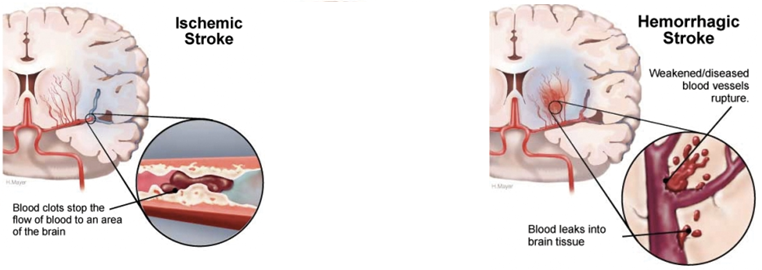
\includegraphics[scale=0.8]{figures/bProblemanalyse/haemoragisk_og_iskaemisk.png}
	\caption{På figuren ses, hvad der sker i encephalon, når henholdsvis iskæmisk og hæmoragisk apopleksi opstår. Der ses til venstre på billedet, at iskæmisk apopleksi sker, hvis en artierie blokkeres. Til højre ses, at hæmoragisk apopleksi opstår, når en arterie brister. \textit{(Revideret)} \cite{Ritter2015}}
	\label{haem-isk}
\end{figure}

\subsubsection{Iskæmisk apopleksi}\label{IskaemiskApp}
Iskæmisk apopleksi opstår i $80-85\%$ af alle apopleksitilfælde \cite{Sundhed.dk2014}. Her blokeres en hjernearterie af en blodprop, der stopper tilførslen af blod til et bestemt område i encephalon, hvilket ses på \figref{haem-isk}. Blodpropperne dannes primært pga. åreforkalkning enten ved en trombe eller en emboli. Trombe sætter sig fast det sted, hvor den er dannet og består af blodplader og fibrin. \cite{Schulze2011} Emboli består typisk af fragmenter af blodceller eller kolesterol, som er diffunderet ind i blodcirkulationen af encephalon fra arterierne \cite{Academic2015a}. Nervecellerne skades efter få minutter grundet iltmangel men kan i værste tilfælde dø efter denne periode \cite{Schulze2011,Giraldo2015}.% grundet iltmangel efter få minutter, og hvis dette fortsætter i en periode, vil de til sidst gå tabt. [5] % Specificer denne periode - hvor lang tid går der, før nervecellen går tabt?

\subsubsection{Hæmoragisk apopleksi}
Hæmoragisk apopleksi opstår i $10-15\%$ af tilfældene iblandt det samlede antal af apopleksiramte \cite{Sundhed.dk2014}. Årsagen heraf skyldes hovedsagligt forhøjet blodtryk eller, i sjældnere tilfælde, aneurismer eller medfødte misdannede kar \cite{Schulze2011}. Hæmoragisk apopleksi opstår, når en hjernearterie brister, og lækage af blod danner en blodansamling, hvilket ses på \figref{haem-isk}. Dette beskadiger det omkringliggende væv og forøger trykket i encephalon. Intracerebral hæmoragi opstår ofte af forhøjet blodtryk, der danner et pres på de små arterier, som får dem til at briste. \cite{Caplan2006}

Blødning i subaraknoidalrummene skyldes ofte bristning af en aneurisme i encephalon \cite{Schulze2011}.\fxnote{NTK: Subaraknoidalrummene er rummet mellem hjernehinderne} Symptomerne ved subaraknoidalblødning er generel tab af hjernefunktion, da der forekommer et øget pres på cerebrum, hvorimod hæmatomet ved intracerebral hæmoragi er lokaliseret et bestemt sted i encephalon og forårsager nedsat funktion af én bestemt hjernefunktion \cite{Caplan2006}. 

%%%%%%%%%%%%%%%%%%%%%%%%%%%%%%%%%%%%%%%%%%%%%%%%%%%%%%%%%%%%%%%%% Gamle ting
%Apopleksi er af World Health Organization (WHO) defineret som pludseligt opstået fokale neurologiske symptomer pga. forstyrrelser i hjernens blodcirkulation, der varer mere end 24 timer eller fører til døden[1gammel].
% [1gammel] = (Experience from a multicentre stroke register: a preliminary report.): http://www.ncbi.nlm.nih.gov/pubmed?cmd=Search&term=Bull%20WHO%20%5Bta%5D%20AND%2054%5Bvol%5D%20AND%20541%5Bpage%5D 